\documentclass[]{article}
\usepackage{lmodern}
\usepackage{amssymb,amsmath}
\usepackage{ifxetex,ifluatex}
\usepackage{fixltx2e} % provides \textsubscript
\ifnum 0\ifxetex 1\fi\ifluatex 1\fi=0 % if pdftex
  \usepackage[T1]{fontenc}
  \usepackage[utf8]{inputenc}
\else % if luatex or xelatex
  \ifxetex
    \usepackage{mathspec}
  \else
    \usepackage{fontspec}
  \fi
  \defaultfontfeatures{Ligatures=TeX,Scale=MatchLowercase}
\fi
% use upquote if available, for straight quotes in verbatim environments
\IfFileExists{upquote.sty}{\usepackage{upquote}}{}
% use microtype if available
\IfFileExists{microtype.sty}{%
\usepackage{microtype}
\UseMicrotypeSet[protrusion]{basicmath} % disable protrusion for tt fonts
}{}
\usepackage[margin=1in]{geometry}
\usepackage{hyperref}
\hypersetup{unicode=true,
            pdftitle={Satellite Image Landcover Classification and Accuracy Assessment using LandSat TM 8 image and the Random Forest Classifier.},
            pdfauthor={James Portolese},
            pdfborder={0 0 0},
            breaklinks=true}
\urlstyle{same}  % don't use monospace font for urls
\usepackage{color}
\usepackage{fancyvrb}
\newcommand{\VerbBar}{|}
\newcommand{\VERB}{\Verb[commandchars=\\\{\}]}
\DefineVerbatimEnvironment{Highlighting}{Verbatim}{commandchars=\\\{\}}
% Add ',fontsize=\small' for more characters per line
\usepackage{framed}
\definecolor{shadecolor}{RGB}{248,248,248}
\newenvironment{Shaded}{\begin{snugshade}}{\end{snugshade}}
\newcommand{\KeywordTok}[1]{\textcolor[rgb]{0.13,0.29,0.53}{\textbf{#1}}}
\newcommand{\DataTypeTok}[1]{\textcolor[rgb]{0.13,0.29,0.53}{#1}}
\newcommand{\DecValTok}[1]{\textcolor[rgb]{0.00,0.00,0.81}{#1}}
\newcommand{\BaseNTok}[1]{\textcolor[rgb]{0.00,0.00,0.81}{#1}}
\newcommand{\FloatTok}[1]{\textcolor[rgb]{0.00,0.00,0.81}{#1}}
\newcommand{\ConstantTok}[1]{\textcolor[rgb]{0.00,0.00,0.00}{#1}}
\newcommand{\CharTok}[1]{\textcolor[rgb]{0.31,0.60,0.02}{#1}}
\newcommand{\SpecialCharTok}[1]{\textcolor[rgb]{0.00,0.00,0.00}{#1}}
\newcommand{\StringTok}[1]{\textcolor[rgb]{0.31,0.60,0.02}{#1}}
\newcommand{\VerbatimStringTok}[1]{\textcolor[rgb]{0.31,0.60,0.02}{#1}}
\newcommand{\SpecialStringTok}[1]{\textcolor[rgb]{0.31,0.60,0.02}{#1}}
\newcommand{\ImportTok}[1]{#1}
\newcommand{\CommentTok}[1]{\textcolor[rgb]{0.56,0.35,0.01}{\textit{#1}}}
\newcommand{\DocumentationTok}[1]{\textcolor[rgb]{0.56,0.35,0.01}{\textbf{\textit{#1}}}}
\newcommand{\AnnotationTok}[1]{\textcolor[rgb]{0.56,0.35,0.01}{\textbf{\textit{#1}}}}
\newcommand{\CommentVarTok}[1]{\textcolor[rgb]{0.56,0.35,0.01}{\textbf{\textit{#1}}}}
\newcommand{\OtherTok}[1]{\textcolor[rgb]{0.56,0.35,0.01}{#1}}
\newcommand{\FunctionTok}[1]{\textcolor[rgb]{0.00,0.00,0.00}{#1}}
\newcommand{\VariableTok}[1]{\textcolor[rgb]{0.00,0.00,0.00}{#1}}
\newcommand{\ControlFlowTok}[1]{\textcolor[rgb]{0.13,0.29,0.53}{\textbf{#1}}}
\newcommand{\OperatorTok}[1]{\textcolor[rgb]{0.81,0.36,0.00}{\textbf{#1}}}
\newcommand{\BuiltInTok}[1]{#1}
\newcommand{\ExtensionTok}[1]{#1}
\newcommand{\PreprocessorTok}[1]{\textcolor[rgb]{0.56,0.35,0.01}{\textit{#1}}}
\newcommand{\AttributeTok}[1]{\textcolor[rgb]{0.77,0.63,0.00}{#1}}
\newcommand{\RegionMarkerTok}[1]{#1}
\newcommand{\InformationTok}[1]{\textcolor[rgb]{0.56,0.35,0.01}{\textbf{\textit{#1}}}}
\newcommand{\WarningTok}[1]{\textcolor[rgb]{0.56,0.35,0.01}{\textbf{\textit{#1}}}}
\newcommand{\AlertTok}[1]{\textcolor[rgb]{0.94,0.16,0.16}{#1}}
\newcommand{\ErrorTok}[1]{\textcolor[rgb]{0.64,0.00,0.00}{\textbf{#1}}}
\newcommand{\NormalTok}[1]{#1}
\usepackage{graphicx,grffile}
\makeatletter
\def\maxwidth{\ifdim\Gin@nat@width>\linewidth\linewidth\else\Gin@nat@width\fi}
\def\maxheight{\ifdim\Gin@nat@height>\textheight\textheight\else\Gin@nat@height\fi}
\makeatother
% Scale images if necessary, so that they will not overflow the page
% margins by default, and it is still possible to overwrite the defaults
% using explicit options in \includegraphics[width, height, ...]{}
\setkeys{Gin}{width=\maxwidth,height=\maxheight,keepaspectratio}
\IfFileExists{parskip.sty}{%
\usepackage{parskip}
}{% else
\setlength{\parindent}{0pt}
\setlength{\parskip}{6pt plus 2pt minus 1pt}
}
\setlength{\emergencystretch}{3em}  % prevent overfull lines
\providecommand{\tightlist}{%
  \setlength{\itemsep}{0pt}\setlength{\parskip}{0pt}}
\setcounter{secnumdepth}{0}
% Redefines (sub)paragraphs to behave more like sections
\ifx\paragraph\undefined\else
\let\oldparagraph\paragraph
\renewcommand{\paragraph}[1]{\oldparagraph{#1}\mbox{}}
\fi
\ifx\subparagraph\undefined\else
\let\oldsubparagraph\subparagraph
\renewcommand{\subparagraph}[1]{\oldsubparagraph{#1}\mbox{}}
\fi

%%% Use protect on footnotes to avoid problems with footnotes in titles
\let\rmarkdownfootnote\footnote%
\def\footnote{\protect\rmarkdownfootnote}

%%% Change title format to be more compact
\usepackage{titling}

% Create subtitle command for use in maketitle
\providecommand{\subtitle}[1]{
  \posttitle{
    \begin{center}\large#1\end{center}
    }
}

\setlength{\droptitle}{-2em}

  \title{Satellite Image Landcover Classification and Accuracy Assessment using
LandSat TM 8 image and the Random Forest Classifier.}
    \pretitle{\vspace{\droptitle}\centering\huge}
  \posttitle{\par}
    \author{James Portolese}
    \preauthor{\centering\large\emph}
  \postauthor{\par}
      \predate{\centering\large\emph}
  \postdate{\par}
    \date{Jan 8, 2020}


\begin{document}
\maketitle

\subsection{Introduction}\label{introduction}

Landcover mapping based on aerial photographs and ground truth survey is
a time consuming process with inherent problems. Large projects require
the acquisition and processing of potentially thousands of aerial photos
depending on the study area. Human interpretation takes many hours and
is subject to human perception and bias. Satellite imagery and machine
learning algorithms, have been used to create landcover maps for use on
a wide variety of environmental projects. Satellite imagery typically
covers large areas meaning a single image can cover most study areas.
Landsat Thematic Mapper imagery can be used to classify landcover but is
limited due to spatial resolution of 30 meters (ground pixel).

This project will use the Random Forest Classifier and selected bands
from a Landsat 8 TM image of Martha's Vineyard Massachusetts to attempt
to predict 9 landcover classes. The prediction will be based on spectral
response across bands 1 - 7 of the image. The training data will be
based polygons that were drawn on areas of known landcover based on
aerial photo interpretation. The polygons will capture the spectral
response of pixels of known landcover and these pixels will be used to
train a model. A smaller subset image of the island of Martha's Vineyard
was subset in order to speed processing and get around large file sizes
for this project. Traning pixels were selected based on know landcover
areas and a model was created based on these training pixels spectral
response to predict landcover. The final model will be used to classify
the entire image and an accuracy assessment will be performed using
landcover ground truth data interpreted from aerial photographs by the
state of Massachusetts Department of Environmental Protection.

\subsection{Dataset Summary}\label{dataset-summary}

Since 1972, the NASA Landsat program has imaged the earth at varying
spectral, and spatial resolutions using a series of satellites. LandSat
8 was launched in 2013 and includes 11 bands of spectral information in
the visible and infrared spectrum. The imaging scanner collects pixels
of reflected light at a fairly course spatial resolution (30 meters
ground sampling unit depending on the band) but this allows large swaths
of the earth to be recorded on a regular basis and provides ready to
analyze images for use in many applications. For this project, I have
acquired a single path/row in the form of individual tiff images for
each reflectance band the satellite covers. Each band is reflectance in
a narrow section of the electromagnetic spectrum. The band/wavelength
breakdown for the bands used in the project and potential uses of each
band are as follows.

\begin{figure}
\centering
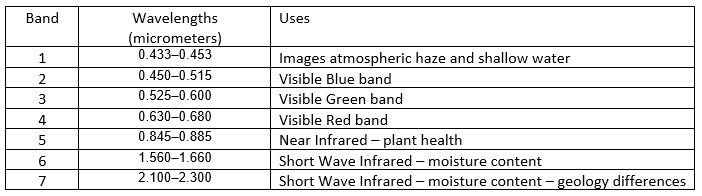
\includegraphics{images/Table1.png}
\caption{Table 1 : Selected Landsat Band Summary}
\end{figure}

The Landsat Thematic Mapper 8 satellite also records additional bands
that I will not use in this project. Bands 8, 9, 10, 11 are of varying
spatial and spectral resolutions but are typically used for additional
visual detail, cloud identification, and Thermal information. A single
Landsat 8 image of Path 012 Row 031 acquired on July 13, 2016 was chosen
for the project. A 2016 image was chosen because a comprehensive
landcover map from 2016 was available to use as ground truth for the
project. A July image was chosen to insure that a significant amount of
vegetation would be visible by the sensor, in hopes that it might allow
for better separation of image landcover classes. The image was
downloaded from the \href{https://earthexplorer.usgs.gov/}{USGS} website

The size of each LandSat Path/Row including all 11 bands is well over
1.5 GB in size. In order to make things more manageable for this project
I acquired the image from the USGS website and pre-processed each bands
tiff image. The images were clipped with a study area feature class
stored in an ESRI file Geodatabase. The result was 7 tiffs with over
1.28 million pixels per image but at a much more reasonable 2MB per
image. As shown in Table 1 each band measures reflectance in a narrow
band of the electromagnetic spectrum. The red green and blue bands
provide info in the visible spectrum but bands 5, 6, and 7 are outside
the human eyes visible range. These bands help with plant
identification, plant health, moisture content and mineral
identification. Overall it is hoped that the spectral response across
all 7 bands will be useful in predicting landcover at the site of each
pixel.

For this project a set of generalized landcover types were used. Table 2
shows the Selected Landcover types used in this project.

\begin{figure}
\centering
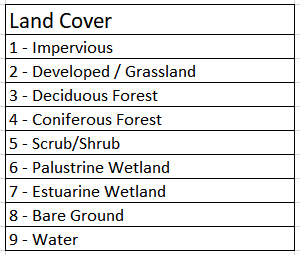
\includegraphics{images/Table2.png}
\caption{Table 2 : Landcover Types Used in this Project}
\end{figure}

Each band used in this project was provided as a single panchromatic
image where the lowest response pixels are black (near 0 reflectance
value) or near black and the highest response are white or near white.
In addition to reflectance values the images are georeferenced meaning
that the pixels are tied to latitude and longitude locations on the
ground. The individual pixels values for each band are stored and so are
coordinates for the center of the pixel. This allows users to drape the
tif images over a map with the necessary software packages. The
classified image can be draped over the 2016 ground truth data for a
pixel to pixel comparison. The data was processed into separate geotiff
files for each band and was imported into a spatial dataframe in r with
the following code:

\begin{Shaded}
\begin{Highlighting}[]
\KeywordTok{library}\NormalTok{(rgdal)}
\KeywordTok{library}\NormalTok{(raster)}
\KeywordTok{library}\NormalTok{(caret)}

\CommentTok{#set subset Image file location}
\NormalTok{path <-}\StringTok{ "./SubsetImagery/"}
\KeywordTok{setwd}\NormalTok{(path)}

\CommentTok{#import each tif file into a spatial grid dataframe}
\NormalTok{new_B1 <-}\StringTok{ }\KeywordTok{readGDAL}\NormalTok{(}\StringTok{"band1.tif"}\NormalTok{)}
\NormalTok{new_B2 <-}\StringTok{ }\KeywordTok{readGDAL}\NormalTok{(}\StringTok{"band2.tif"}\NormalTok{)}
\NormalTok{new_B3 <-}\StringTok{ }\KeywordTok{readGDAL}\NormalTok{(}\StringTok{"band3.tif"}\NormalTok{)}
\NormalTok{new_B4 <-}\StringTok{ }\KeywordTok{readGDAL}\NormalTok{(}\StringTok{"band4.tif"}\NormalTok{)}
\NormalTok{new_B5 <-}\StringTok{ }\KeywordTok{readGDAL}\NormalTok{(}\StringTok{"band5.tif"}\NormalTok{)}
\NormalTok{new_B6 <-}\StringTok{ }\KeywordTok{readGDAL}\NormalTok{(}\StringTok{"band6.tif"}\NormalTok{)}
\NormalTok{new_B7 <-}\StringTok{ }\KeywordTok{readGDAL}\NormalTok{(}\StringTok{"band7.tif"}\NormalTok{)}
\end{Highlighting}
\end{Shaded}

The import (readGDAL) makes use of several R libraries specifically the
rgdal and raster packages. These must be loaded in order to import the
individual tif files. After the upload is complete, each band is stored
in a spatial grid data frame.

The code below displays a single band (spatial grid dataframe) using the
plot command.

\begin{Shaded}
\begin{Highlighting}[]
\KeywordTok{plot}\NormalTok{(new_B5,}\DataTypeTok{col =} \KeywordTok{gray}\NormalTok{(}\DecValTok{0}\OperatorTok{:}\DecValTok{100} \OperatorTok{/}\StringTok{ }\DecValTok{100}\NormalTok{))}
\end{Highlighting}
\end{Shaded}

\begin{figure}
\centering
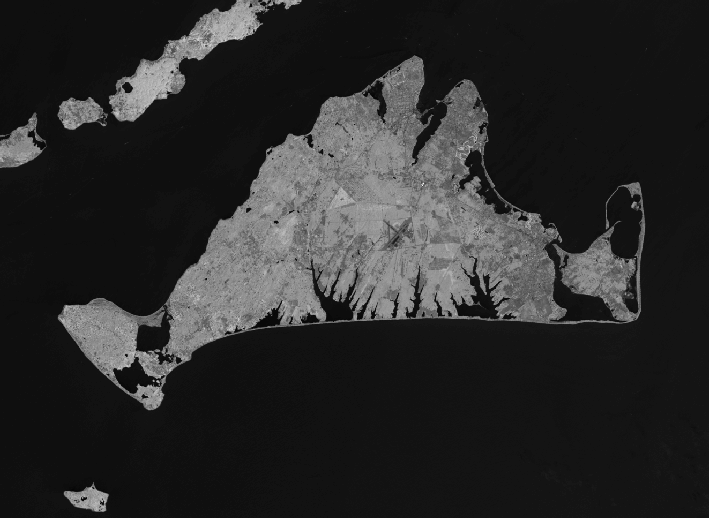
\includegraphics{images/Band5.png}
\caption{Figure 3: Panchromatic Band 5 (Near Infrared) of Study Area}
\end{figure}

Once each tif file is imported into a spatial grid dataframe each
individual dataframe is converted into a raster layer and then stacked
into a single raster stack with 7 dimensions using the code below.

\begin{Shaded}
\begin{Highlighting}[]
\NormalTok{FullImage <-}\StringTok{ }\KeywordTok{stack}\NormalTok{(}\KeywordTok{raster}\NormalTok{(new_B1), }\KeywordTok{raster}\NormalTok{(new_B2), }\KeywordTok{raster}\NormalTok{(new_B3)}
\NormalTok{                   , }\KeywordTok{raster}\NormalTok{(new_B4), }\KeywordTok{raster}\NormalTok{(new_B5), }\KeywordTok{raster}\NormalTok{(new_B6), }
                   \KeywordTok{raster}\NormalTok{(new_B7))}

\CommentTok{# update the names of the raster stack to a simpler B1 - B7}
\KeywordTok{names}\NormalTok{(FullImage) <-}\StringTok{ }\KeywordTok{paste0}\NormalTok{(}\StringTok{"B"}\NormalTok{, }\KeywordTok{c}\NormalTok{(}\DecValTok{1}\OperatorTok{:}\DecValTok{7}\NormalTok{))}
\end{Highlighting}
\end{Shaded}

The result is a raster stack with dimensions of 724 rows and 1132
columns. The image has a total of 819,568 pixels and 7 layers (one for
each band B1 - B7). The original image (full size image before study
area clipping) was 8011 rows and 7901 columns (63,294,911 pixels).
Landsat imagery can be quite cumbersome to store and handle and for this
reason for this project I used a smaller subset that centered on the
island of Martha's Vineyard.

An image can be Visually interpreted using the computer screen. A single
panchromatic band (layer) is mapped to the blue, red, or green display
of the computer screen and in combination with other bands results in a
raster stack that can be viewed and intepreted. A true color image can
be displayed by matching band 4 to red, band 3 to green and band 2 to
blue. (4,3,2).

A true color image can be stacked with the following code:

\begin{Shaded}
\begin{Highlighting}[]
\KeywordTok{plotRGB}\NormalTok{(FullImage }\OperatorTok{*}\StringTok{ }\NormalTok{(FullImage }\OperatorTok{>=}\StringTok{ }\DecValTok{0}\NormalTok{)}
\NormalTok{        , }\DataTypeTok{r =} \DecValTok{4}\NormalTok{, }\DataTypeTok{g =} \DecValTok{3}\NormalTok{, }\DataTypeTok{b =} \DecValTok{2}
\NormalTok{        , }\DataTypeTok{stretch =}\StringTok{'lin'}\NormalTok{)}
\end{Highlighting}
\end{Shaded}

\begin{figure}
\centering
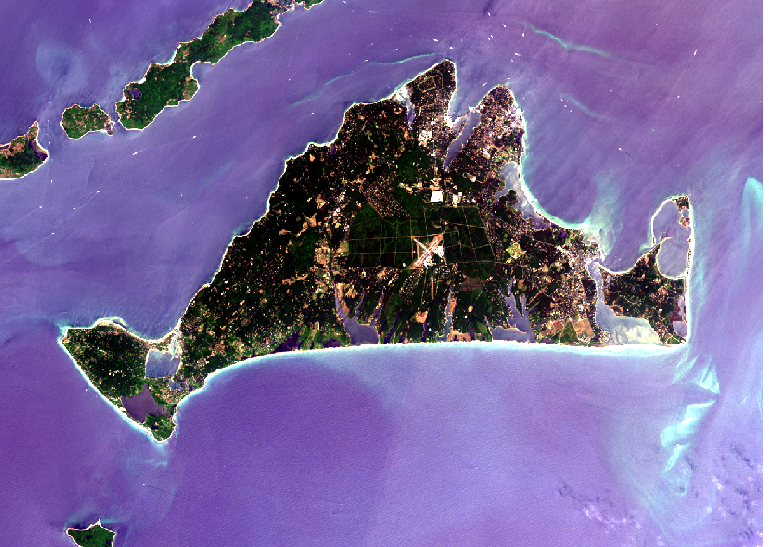
\includegraphics{images/TrueColor_MV.png}
\caption{\textbf{\emph{Figure 4: Stretched True Color Image Martha's
Vineyard Subset using bands 4,3,2}}}
\end{figure}

While the near infrared and short wave infrared bands are not in the
range of light the eye can see, we can create a pseudo color image using
the screen colors and map the NIR and SWIR bands to the visible red,
green, or blue display of the computer screen and visually interpret the
image.

The following code creates a false color image:

\begin{Shaded}
\begin{Highlighting}[]
\KeywordTok{plotRGB}\NormalTok{(FullImage }\OperatorTok{*}\StringTok{ }\NormalTok{(FullImage }\OperatorTok{>=}\StringTok{ }\DecValTok{0}\NormalTok{)}
\NormalTok{        , }\DataTypeTok{r =} \DecValTok{5}\NormalTok{, }\DataTypeTok{g =} \DecValTok{4}\NormalTok{, }\DataTypeTok{b =} \DecValTok{3}
\NormalTok{        , }\DataTypeTok{scale =} \DecValTok{2}
\NormalTok{        , }\DataTypeTok{stretch =}\StringTok{'lin'}\NormalTok{)}
\end{Highlighting}
\end{Shaded}

\begin{figure}
\centering
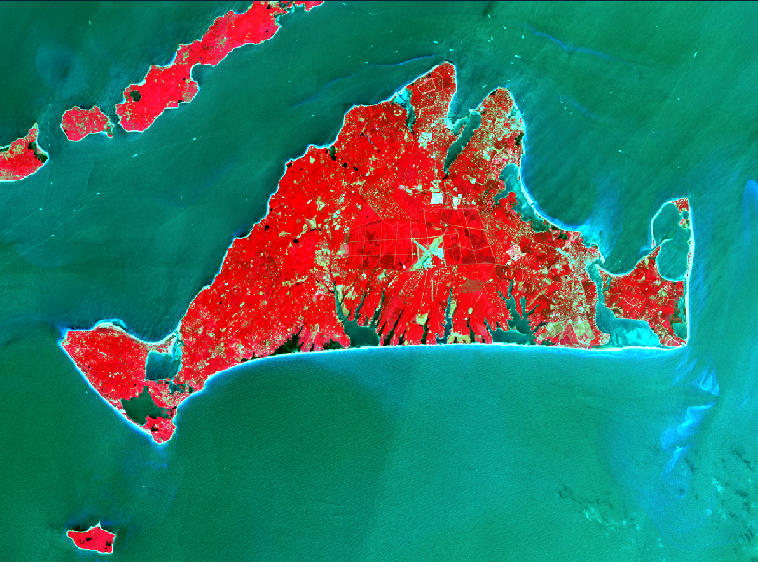
\includegraphics{images/CIR_MV.png}
\caption{\textbf{\emph{Figure 5 : A false color infrared image Band 5
(Near IR), Band 4 (Red), Band 3 (Green) of the Martha's Vineyard subset.
This image highlights the Near Infrared reflectance (vegetation) in
red.}}}
\end{figure}

\subsection{Methodology - Model Creation and Training
Methodology}\label{methodology---model-creation-and-training-methodology}

After processing the input data and importing it into R the next step
was to identify training areas on the image that identify known
landcover types.

Again the landcover types I am attempting to predict are the following:

Impervious Surfaces\\
Developed Open areas / Grassland\\
Deciduous Forest\\
Coniferous Forest\\
Scrub/Shrub\\
Palustrine Wetland (Non salt water wetland)\\
Estuarine Wetland (salt water wetland)\\
Bare Ground (Sand, Exposed Dirt)\\
Water

The first step in creating the model was to collect pixel reflectance
values for areas of known landcover (training areas). Since the imagery
is georeferenced to locations on the ground we can use other
georeferenced imagery (in this case aerial photographs) to identify
suitable training areas of the known landcover classes in this project.
Training polygons for the study were acquired for each landcover type
using aerial photo interpretation. Polygons were drawn in GIS software
to capture pixels of known landcover and their reflectance values were
stored. The polygons were stored in a ESRI feature class and will be
imported into R as a spatial polygons dataframe (using rgdal / ogr) the
polygons were used to extract pixels from the study area image.

The polygons are included in the file geodatabase provided in the github
repository for this project

A few of of the training polygons are shown in Figures 6, 7, and 8,
below:

\begin{figure}
\centering
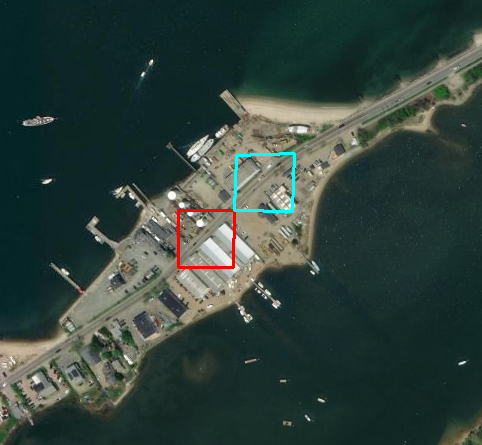
\includegraphics{images/ImpTA.png}
\caption{\textbf{\emph{Figure 6 : Impervious Surface Training
Polygons}}}
\end{figure}

\begin{figure}
\centering
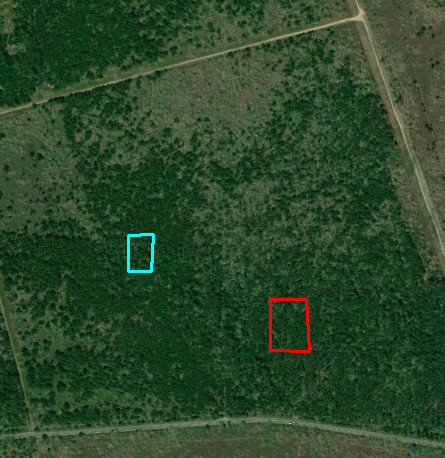
\includegraphics{images/CF_TA.png}
\caption{\textbf{\emph{Figure 7: Coniferous Forest Training Area}}}
\end{figure}

\begin{figure}
\centering
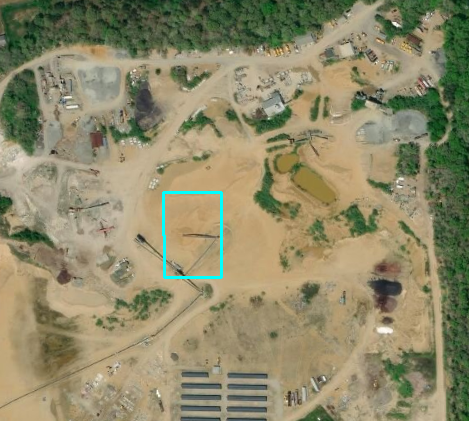
\includegraphics{images/BG_TA.png}
\caption{\textbf{\emph{Figure 8 : Bare Ground Training Area}}}
\end{figure}

Training polygons were identified over areas of pure landcover and the
polygons were used to extract reflectance information over the much
coarser resolution (30 meter pixel) Satellite image used in the project.

The final set of training polygons was imported into R with the
following code:

\begin{Shaded}
\begin{Highlighting}[]
\NormalTok{fgdb <-}\StringTok{ "../GISData.gdb"}  \CommentTok{# set the location of the file geodatabase}
\NormalTok{TrainingPixels <-}\StringTok{ }\KeywordTok{readOGR}\NormalTok{(}\DataTypeTok{dsn=}\NormalTok{fgdb, }\StringTok{"MVTrainingAreas"}\NormalTok{)}
\end{Highlighting}
\end{Shaded}

The result is a spatial Polygons dataframe that identifies areas on the
ground that correspond to the 9 landcover types we are attempting to
identify.\\
This set of polygons was used to pull reflectance values from the
satellite image across all 7 bands. The 7 bands of reflectance values
were pulled from pixels that fell inside the training areas. These
values were input into a dataframe.

The following code creates a dataframe that holds the pixel values and a
class number for each of the above landcover types

\begin{Shaded}
\begin{Highlighting}[]
\NormalTok{responseCol <-}\StringTok{ "CovCode"}

\NormalTok{dfTraining =}\StringTok{ }\KeywordTok{data.frame}\NormalTok{(}\KeywordTok{matrix}\NormalTok{(}\KeywordTok{vector}\NormalTok{(), }\DataTypeTok{nrow =} \DecValTok{0}\NormalTok{, }\DataTypeTok{ncol =} \KeywordTok{length}\NormalTok{(}\KeywordTok{names}\NormalTok{(FullImage)) }\OperatorTok{+}\StringTok{ }\DecValTok{1}\NormalTok{))   }
\ControlFlowTok{for}\NormalTok{ (i }\ControlFlowTok{in} \DecValTok{1}\OperatorTok{:}\KeywordTok{length}\NormalTok{(}\KeywordTok{unique}\NormalTok{(TrainingPixels[[responseCol]])))\{}
\NormalTok{  category <-}\StringTok{ }\KeywordTok{unique}\NormalTok{(TrainingPixels[[responseCol]])[i]}
\NormalTok{  categorymap <-}\StringTok{ }\NormalTok{TrainingPixels[TrainingPixels[[responseCol]] }\OperatorTok{==}\StringTok{ }\NormalTok{category,]}
\NormalTok{  dataSet <-}\StringTok{ }\NormalTok{raster}\OperatorTok{::}\KeywordTok{extract}\NormalTok{(FullImage, categorymap)}
\NormalTok{  dataSet <-}\StringTok{ }\NormalTok{dataSet[}\OperatorTok{!}\KeywordTok{unlist}\NormalTok{(}\KeywordTok{lapply}\NormalTok{(dataSet, is.null))]}
\NormalTok{  dataSet <-}\StringTok{ }\KeywordTok{lapply}\NormalTok{(dataSet, }\ControlFlowTok{function}\NormalTok{(x)\{}\KeywordTok{cbind}\NormalTok{(x, }\DataTypeTok{class =} \KeywordTok{as.numeric}\NormalTok{(}\KeywordTok{rep}\NormalTok{(category, }\KeywordTok{nrow}\NormalTok{(x))))\})}
\NormalTok{  df <-}\StringTok{ }\KeywordTok{do.call}\NormalTok{(}\StringTok{"rbind"}\NormalTok{, dataSet)}
\NormalTok{  dfTraining <-}\StringTok{ }\KeywordTok{rbind}\NormalTok{(dfTraining, df)}
\NormalTok{\}}
\end{Highlighting}
\end{Shaded}

dfTraining is a dataframe of 679 pixels across the various landcover
types. Each row of the dataframe includes reflectance values for a
single image pixel across each of the 7 bands as well as a class column
to identify which landcover type it belongs to.

This data will be used to train the model but before we do it is good
practice to see how consistent the pixels are spectrally for each
landcover training area. In order to identify outliers or
inconsistencies in the training area pixels plots were made to show the
response of all pixels for each landcover across all 7 bands. Each plot
is a different landcover and each plot line is an individual pixel area.

The following code was used to generate plots.

\begin{Shaded}
\begin{Highlighting}[]
\NormalTok{###############################################################################}
\CommentTok{#Analyze and plot training set pixels.}

\KeywordTok{library}\NormalTok{(ggplot2)}
\KeywordTok{library}\NormalTok{(dplyr)}

\CommentTok{# add an ID to each pixel in the training }
\CommentTok{# dataframe for plotting}

\CommentTok{# add an ID to dfTraining for plotting}
\NormalTok{ID =}\StringTok{ }\KeywordTok{seq}\NormalTok{(}\DecValTok{1}\OperatorTok{:}\KeywordTok{nrow}\NormalTok{(dfTraining))}
\NormalTok{dfTraining <-}\StringTok{ }\KeywordTok{cbind}\NormalTok{(dfTraining, ID)}

\CommentTok{# load simple lookup table created in excel for the landcover classes and merge}
\CommentTok{#df training to show the class names in the final plot}
\NormalTok{lookup <-}\StringTok{ }\KeywordTok{read.csv}\NormalTok{(}\DataTypeTok{file=}\StringTok{"../lookup.csv"}\NormalTok{, }\DataTypeTok{header=}\OtherTok{TRUE}\NormalTok{)}
\NormalTok{TrainingSignatures <-}\StringTok{ }\KeywordTok{merge}\NormalTok{(dfTraining, lookup, }\DataTypeTok{by.x =} \StringTok{"class"}\NormalTok{, }\DataTypeTok{by.y=}\StringTok{"LCID"}\NormalTok{)}

\KeywordTok{ncol}\NormalTok{(lookup)}

\CommentTok{# load tidyverse to use the gather command}
\KeywordTok{library}\NormalTok{(tidyr)}

\NormalTok{TrainingSignatures }\OperatorTok\StringTok{ }
\StringTok{  }\KeywordTok{gather}\NormalTok{(col, val, }\OperatorTok{-}\KeywordTok{c}\NormalTok{(classname, ID, class)) }\OperatorTok\StringTok{  }\CommentTok{# from `tidyr`}
\StringTok{  }\KeywordTok{ggplot}\NormalTok{(}\KeywordTok{aes}\NormalTok{(col, val, }\DataTypeTok{color =}\NormalTok{ ID, }\DataTypeTok{group =}\NormalTok{ ID)) }\OperatorTok{+}\StringTok{ }
\StringTok{  }\KeywordTok{geom_line}\NormalTok{() }\OperatorTok{+}
\StringTok{  }\KeywordTok{facet_wrap}\NormalTok{(}\OperatorTok{~}\NormalTok{classname)}


\NormalTok{########################################################}
\end{Highlighting}
\end{Shaded}

The resulting plots are show below.

\begin{figure}
\centering
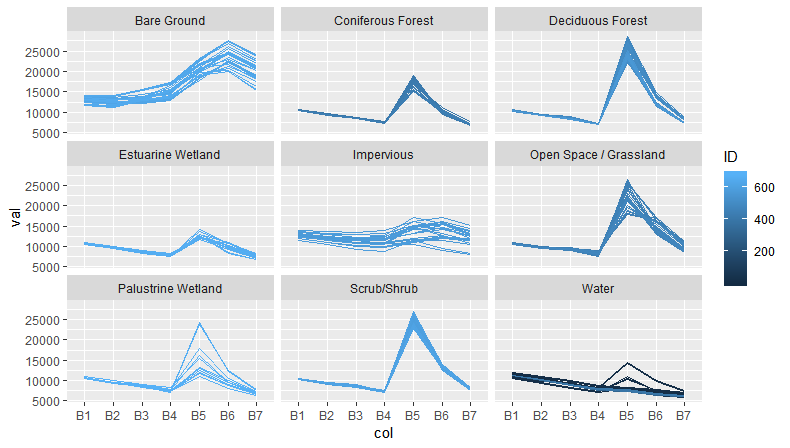
\includegraphics{images/TrainingSetPlot.png}
\caption{\textbf{\emph{Figure 9 - Training set pixels plotted by land
cover type}}}
\end{figure}

Each plot is a single landcover type and each separate line plots a
single pixels reflectance values across all 7 bands.

A few comments on these plots:

The first plot (Bare Ground) shows a fairly consistent shape but with
high pixel variation in each band. The pixels follow a consistent trend
but vary widely in value

Coniferous Forest pixels look very similar to Deciduous forest except
for a lower reflectance in bands 5 amd 6.

Scrub Shrub and Deciduous Forest training pixels look very similar
spectrally.

Water has a clear variation in that some pixels show higher reflectance
in Bands 4 - 6. These bands are in the near infrared and infrared
portion of the spectrum. I would assume that this is due to shallow
vs.~deep water reflectance.

The more consistent shape and tighter the pixel response the better the
training area but in some cases variation exists due to mixed pixels.

The model is only as good as the training pixels while there are some
potential issues with the training set we will next move forward to
training the model

\subsection{Landcover Model Creation Using Random
Forest}\label{landcover-model-creation-using-random-forest}

Random Forest is one of the most widely used ensemble classification
algorithms. It uses a series of decision trees to make predictions.
Separate decision trees each based on subsets of predictors and training
pixels attempt to predict the landcover class for each training pixel.
The class assigned is based on majority vote of all the trees involved.
For this project I used the Random Forest algorithm for prediction. The
results in the training stage showed a good fit between training pixels
and the model results. The accuracy assesment portion of this document
will outline how close the model was in predicting the landcover in the
pixels outside the training areas.

dfTraining (our training data set) is only a tiny subset (693 pixels) of
the entire study area image (724 x 1132 or 819,568 pixels).

Using the dfTraining dataframe created in the earlier section of this
report, I used the following code to create the model. In order to use
the random forest algorithm I loaded the caret package in R

\begin{Shaded}
\begin{Highlighting}[]
\CommentTok{# apply randomforest to training set.  Using all 7 bands  }
\KeywordTok{library}\NormalTok{(caret)}
\NormalTok{rfmod1_}\DecValTok{7}\NormalTok{ <-}\StringTok{ }\KeywordTok{train}\NormalTok{(}\KeywordTok{as.factor}\NormalTok{(class)}\OperatorTok{~}\StringTok{ }\NormalTok{B1 }\OperatorTok{+}\StringTok{ }\NormalTok{B2 }\OperatorTok{+}\StringTok{ }\NormalTok{B3 }\OperatorTok{+}\StringTok{ }\NormalTok{B4 }\OperatorTok{+}\StringTok{ }\NormalTok{B5 }\OperatorTok{+}\StringTok{ }\NormalTok{B6 }\OperatorTok{+}\StringTok{ }\NormalTok{B7, }\DataTypeTok{method =} \StringTok{"rf"}\NormalTok{, }\DataTypeTok{data =}\NormalTok{ dfTraining)}
\NormalTok{rfmod1_}\DecValTok{7}
\end{Highlighting}
\end{Shaded}

The 9 classes were stored as numbers:

1 - Impervious 2 - Developed / Grassland\\
3 - Deciduous Forest\\
4 - Conferous Forest\\
5 - Scrub/Shrub\\
6 - Palustrine Wetland\\
7 - Estuarine Wetland\\
8 - Bare Ground\\
9 - Water

Here are the results of running the Random Forest algorithm

693 samples 7 predictor 9 classes: `1', `2', `3', `4', `5', `6', `7',
`8', `9'

No pre-processing Resampling: Bootstrapped (25 reps) Summary of sample
sizes: 693, 693, 693, 693, 693, 693, \ldots{} Resampling results across
tuning parameters:

mtry Accuracy Kappa\\
2 0.9721495 0.9552781 4 0.9738211 0.9580107 7 0.9714812 0.9542984

Accuracy was used to select the optimal model using the largest value.
The final value used for the model was mtry = 4.

The model created decision trees based on subsets of the 7 bands of info
(7 predictors) and 693 training pixels (samples) to predict 9 classes.
The training pixels generated an accuracy of .9715 and a Kappa of .9544
and performed best when mtry = 4 (4 Randomly Selected Predictors)

\begin{figure}
\centering
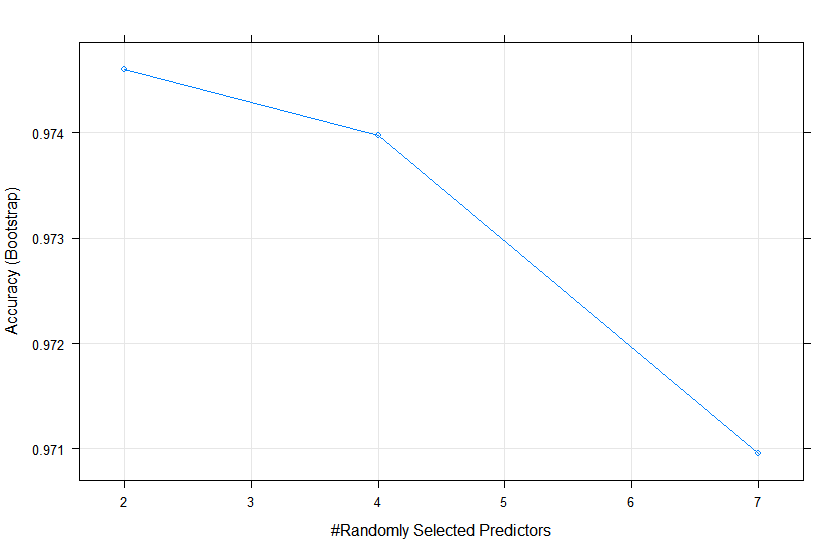
\includegraphics{images/modelPlot.png}
\caption{\textbf{\emph{Figure 10 : Model Plot Accuracy vs.~Number of
Predictors}}}
\end{figure}

Once satisfactory accuracies were achieved the next step was to use the
model to classify landcover across all 800,000+ pixels in the full
image. That was done with the following code.

\begin{Shaded}
\begin{Highlighting}[]
\CommentTok{# Once the model is complete we can use it to classify all pixels in the image}
\NormalTok{LC_Pred_MV <-}\StringTok{ }\KeywordTok{predict}\NormalTok{(FullImage, }\DataTypeTok{model =}\NormalTok{ rfmod1_}\DecValTok{7}\NormalTok{)}
\end{Highlighting}
\end{Shaded}

\subsection{Results - Accuracy
Assessment}\label{results---accuracy-assessment}

While the model accuracy appears to be satisfactory the accuracy of the
predictions in the final classified image had to be assessed. Because of
the wide variation in pixel totals per landcover class in the image, a
proportional stratified random sample was used. A set of random points
needed to be generated on the final image and then checked against
ground truth information to see if the predicted landcover actually is
found at that location.

The final classification using the model (LC\_Pred\_MC in the code) is a
723 x 1131 raster layer that has a single value, predicted landcover
class based on our random forest model. The image with colors assigned
to each landcover class is shown here:

\begin{figure}
\centering
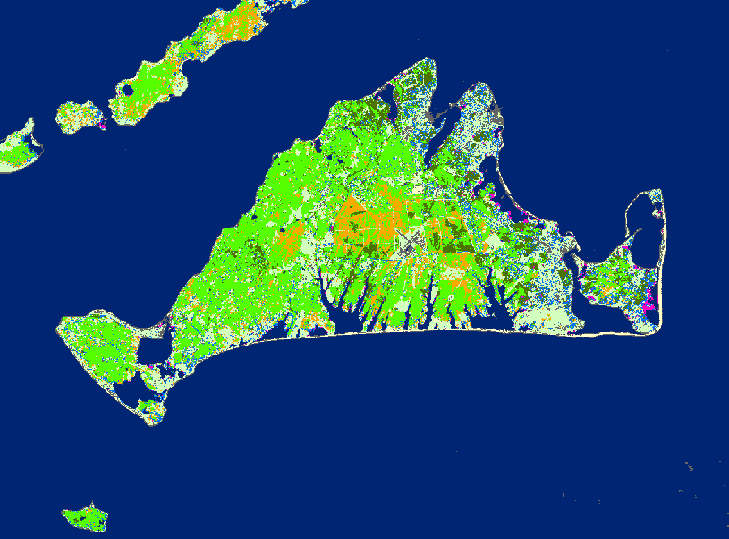
\includegraphics{images/finalClassImg.png}
\caption{\textbf{\emph{Figure 11 : Final Classified Image}}}
\end{figure}

Image classification requires ground truth data in order to effectively
determine the prediction accuracy. Ground truth data is not always easy
to acquire. Random pixels are chosen and landcover is determined by
either visiting the locations on the ground, intepreting aerial
photography acquired during the same time frame as the image (if it
exists and is available), or by using other data sources. In this case,
a newly acquired landcover layer from the State of Massachusetts was
available (it's vintage (2016) guided me in the original image
acquisition). The landcover layer was a series of vector polygons that
were interpreted from 2016 aerial imagery and digitized by the state. I
subset a piece of this data that covered the study area of this project.
I converted the vector polygons to a raster image at 30 meter resolution
to match the Landsat image using GIS software. Once I had the image in
this format I output it into the file geodatabase stored in the github
repository. I imported the image into R with this code:

\begin{Shaded}
\begin{Highlighting}[]
\CommentTok{# import the ground truth image for actual interpreted landcover in the test area}
\NormalTok{GrndTruthImg <-}\StringTok{ }\KeywordTok{readGDAL}\NormalTok{(}\StringTok{"../GroundTruth/GroundTruth_clip3.tif"}\NormalTok{)}
\KeywordTok{plot}\NormalTok{(GrndTruthImg, }\DataTypeTok{col =}\NormalTok{ colors)}
\end{Highlighting}
\end{Shaded}

The newly imported Ground Truth Image was plotted using the same color
scheme and is in the figure below:

\begin{figure}
\centering
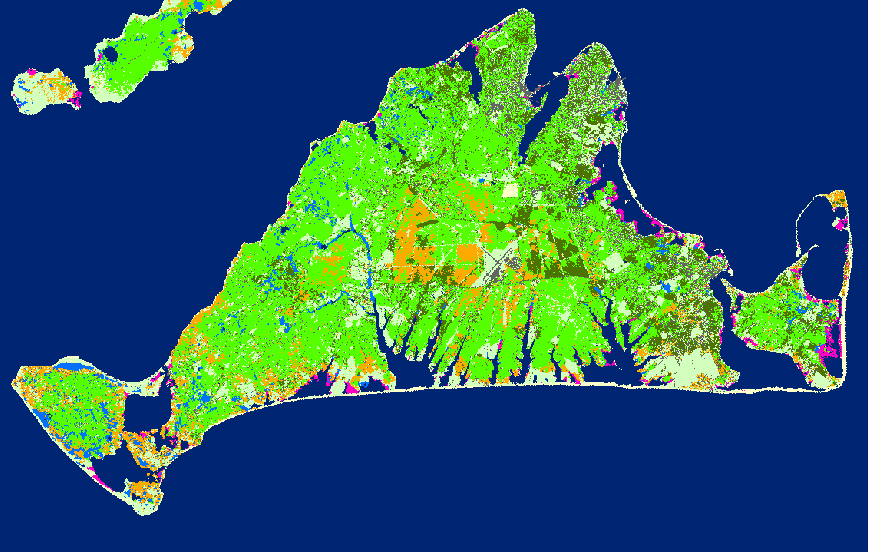
\includegraphics{images/GroundTruth.png}
\caption{\textbf{\emph{Figure 12 : Ground Truth Image}}}
\end{figure}

Now that the Truth image and the predictions image are created a set of
sample points must be generated to compare the prediction vs.~the Truth.
A proportional stratified random sample methodology was used to assess
the accuracy. Proportions of the individual landcovers vs.~the entire
image were calculated and a set of stratified random points were created
on the classified image. The same points were used to extract landcover
information from the Ground Truth Image.

Proportional Totals were calculated by converting the images to vectors
and running the following code:

\begin{Shaded}
\begin{Highlighting}[]
\CommentTok{# Generate a proportions for each classified landcover for use}
\CommentTok{# in a proportional Stratified Random Sample for Accuracy Assessment}

\CommentTok{#Determine how many pixel of each landcover in my classified image}
\NormalTok{imgVector <-}\StringTok{ }\KeywordTok{as.vector}\NormalTok{(FinalClassImg}\OperatorTok{$}\NormalTok{layer)}
\NormalTok{totByLandCover <-}\StringTok{ }\KeywordTok{as.vector}\NormalTok{(}\KeywordTok{table}\NormalTok{(imgVector))}

\CommentTok{# Get the total pixels in the image}
\NormalTok{totalPixels <-}\StringTok{ }\KeywordTok{length}\NormalTok{(imgVector)}

\CommentTok{# Get the percentage of all pixels in each landcover class}
\NormalTok{pixProps <-}\StringTok{ }\NormalTok{totByLandCover }\OperatorTok{/}\StringTok{ }\NormalTok{totalPixels}

\CommentTok{# Choose 5000 total samples}
\NormalTok{TotalSamplePixels <-}\StringTok{ }\DecValTok{5000}
\CommentTok{# calculate the total sample pixels to request for each landcover type}
\NormalTok{PropofTotalsample <-}\StringTok{ }\NormalTok{pixProps }\OperatorTok{*}\StringTok{ }\NormalTok{TotalSamplePixels}

\CommentTok{# Convert to integer to lose the decimal (partial sample)}
\NormalTok{SampleTotals <-}\StringTok{ }\KeywordTok{as.integer}\NormalTok{(PropofTotalsample)}
\end{Highlighting}
\end{Shaded}

A total of 5000 pixels were used in this assessment and the SampleTotals
variable was used to store the totals for each landcover type

The next step was to generate the sample set using this code. A function
that selected the sample points for each individual landcover had to be
written and the two vectors (landcover categories and total samples -
based on the proportions calculated) were passed. The final variable
strat is a dataframe that includes the x y coordinates of the location
and the predicted landcover.

\begin{Shaded}
\begin{Highlighting}[]
\CommentTok{# Write a function to pull n samples from category c so I can pass a }
\CommentTok{# vector of n (total number of samples) and a vector of categories}

\NormalTok{sampleNfromC =}\StringTok{ }\ControlFlowTok{function}\NormalTok{(r,N,C)\{}
\NormalTok{  d=}\KeywordTok{subset}\NormalTok{(}
    \KeywordTok{data.frame}\NormalTok{(}
      \KeywordTok{sampleStratified}\NormalTok{(r}\OperatorTok{==}\NormalTok{C,N, }\DataTypeTok{sp =}\NormalTok{ T)),}
\NormalTok{    layer}\OperatorTok{==}\DecValTok{1}\NormalTok{)}
\NormalTok{  d}\OperatorTok{$}\NormalTok{layer=C}
\NormalTok{  d\}}

\NormalTok{landcovers <-}\StringTok{ }\KeywordTok{as.vector}\NormalTok{(}\KeywordTok{c}\NormalTok{(}\DecValTok{1}\NormalTok{,}\DecValTok{2}\NormalTok{,}\DecValTok{3}\NormalTok{,}\DecValTok{4}\NormalTok{,}\DecValTok{5}\NormalTok{,}\DecValTok{6}\NormalTok{,}\DecValTok{7}\NormalTok{,}\DecValTok{8}\NormalTok{,}\DecValTok{9}\NormalTok{))}
\NormalTok{TotalSamples <-}\StringTok{ }\KeywordTok{as.numeric}\NormalTok{(SampleTotals)  }\CommentTok{# from earlier proportion calculation}

\CommentTok{# pull the samples for each category into a dataframe }
\NormalTok{strat =}\StringTok{ }\KeywordTok{do.call}\NormalTok{(rbind, }\KeywordTok{lapply}\NormalTok{(}\DecValTok{1}\OperatorTok{:}\DecValTok{9}\NormalTok{, }\ControlFlowTok{function}\NormalTok{(i)\{}\KeywordTok{sampleNfromC}\NormalTok{(FinalClassImg, TotalSamples[i],landcovers[i])\}))}
\end{Highlighting}
\end{Shaded}

Strat was converted to a spatial points dataframe and overlain onto the
Ground Truth Image in order to get the actual landcover (based on the
State of Massachusetts interpretation). This code was used to plot the
points.

\begin{Shaded}
\begin{Highlighting}[]
\CommentTok{# convert the samples to a spatial points dataframe }
\NormalTok{coords <-}\StringTok{ }\NormalTok{strat[, }\KeywordTok{c}\NormalTok{(}\StringTok{"x"}\NormalTok{, }\StringTok{"y"}\NormalTok{)]}
\NormalTok{data <-}\StringTok{ }\NormalTok{strat}
\NormalTok{crs <-}\StringTok{ }\KeywordTok{CRS}\NormalTok{(}\StringTok{"+init=epsg:32619"}\NormalTok{)}

\NormalTok{spdf <-}\StringTok{ }\KeywordTok{SpatialPointsDataFrame}\NormalTok{(}\DataTypeTok{coords =}\NormalTok{ coords,}
                               \DataTypeTok{data =}\NormalTok{ data,}
                               \DataTypeTok{proj4string =}\NormalTok{ crs)}

\CommentTok{# plot the samnple locations over the Final Classified Image}
\KeywordTok{plot}\NormalTok{(FinalClassImg, }\DataTypeTok{col =}\NormalTok{ colors, }\DataTypeTok{legend =} \OtherTok{FALSE}\NormalTok{)}
\KeywordTok{points}\NormalTok{(spdf, }\DataTypeTok{pch =} \StringTok{"+"}\NormalTok{)}
\end{Highlighting}
\end{Shaded}

\begin{figure}
\centering
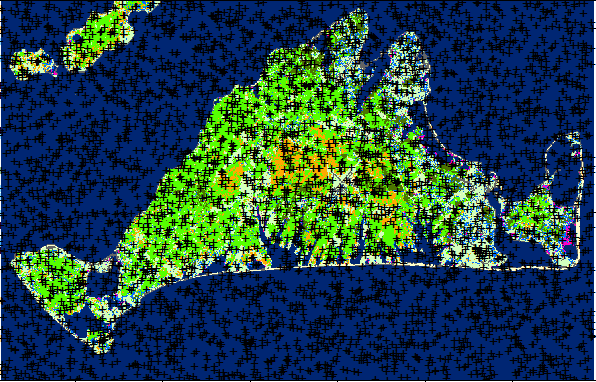
\includegraphics{images/Samples.png}
\caption{\textbf{\emph{Figure 13 : Accuracy Assessment points}}}
\end{figure}

The same locations were applied to the Ground Truth Data and the actual
landcover was extracted with the following code:

\begin{Shaded}
\begin{Highlighting}[]
\NormalTok{#### Convert Ground truth image to a raster from a spatial grid dataframe}
\NormalTok{rast <-}\StringTok{ }\KeywordTok{raster}\NormalTok{(GrndTruthImg)}
\CommentTok{# use sample locations (spdf) to pull Ground truth landcover for comparison}
\NormalTok{GrndTruth <-}\StringTok{ }\NormalTok{raster}\OperatorTok{::}\KeywordTok{extract}\NormalTok{(rast, spdf)}
\end{Highlighting}
\end{Shaded}

The final step was to create a confusion matrix which required GrndTruth
and spdf as vectors for direct comparisons using the confusion matrix
command.

\begin{Shaded}
\begin{Highlighting}[]
\NormalTok{predictions =}\StringTok{ }\KeywordTok{as.vector}\NormalTok{(}\KeywordTok{as.integer}\NormalTok{((spdf}\OperatorTok{$}\NormalTok{layer)))}
\NormalTok{Truth <-}\StringTok{ }\KeywordTok{as.vector}\NormalTok{(}\KeywordTok{as.integer}\NormalTok{((GrndTruth)))}
\KeywordTok{confusionMatrix}\NormalTok{(}\KeywordTok{table}\NormalTok{(Truth,predictions))}
\end{Highlighting}
\end{Shaded}

A reformated confusion matrix is below

\begin{figure}
\centering
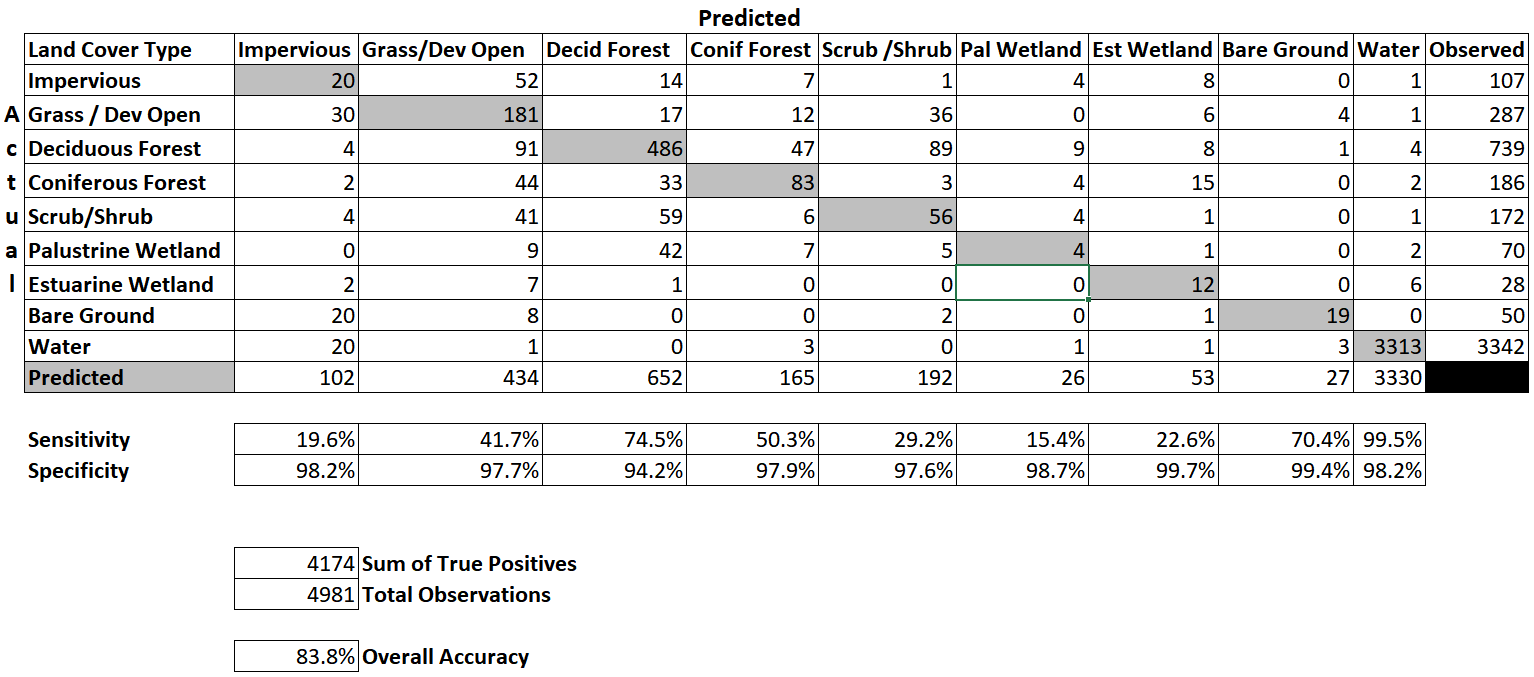
\includegraphics{images/ConfMatrix.png}
\caption{\textbf{\emph{Figure 14 : Confusion Matrix}}}
\end{figure}

\subsection{Conclusions}\label{conclusions}

Overall the Accuracy of the predictions across all of the 5000 samples
was 83.6\%. Some of the individual landcover accuracies were quite poor.
Impervious at 16\% was often confused with Bare Ground as well as water.
This might be expected as sand and concrete have similar spectral
signatures. Deciduous Forest performed well but confusion exists between
it and coniferous forest as well as Scrub/Shrub. Water was by far the
most accurate at 99\% and it also made up a significant amount of the
image. This helped the overall accuracy. The worst performing landcover
was \#6 Palustrine Wetland at 3\%. This landcover is a considerable mix
of water, and different vegetation types so it was hard to identify pure
pixels for training the model that didn't spectrally resemble other
landcover types. Wetlands in general didn't perform well.

The coarse spatial resolution and over enthusiastic choice of landcovers
(too specific) probably led to poor accuracies. A 30m area on the ground
often contains considerable variation in landcover types. Also the
nature of some of the landcovers chosen may themselves contain some
built in confusion. The Developed / Grassland class is not a pure
landcover as it contains housing, lawns and an occasional brush or tree.
Mixed pixels are a problem in all coarse spatial resolution data and
this project is no different.

Overll the project was a great exercise in processing, creating a model,
and accuracy assessing landcover classification in R. Additional time
could be spent working on the training polygons to be sure pure
landcover is being represented and to be sure the training sets were
balanced.


\end{document}
